%# -*- coding: utf-8-unix -*-

\documentclass[project, fontset=adobe, openany, oneside, submit]{sjtuthesis}
\addbibresource{bib/thesis.bib}
\begin{document}

% ========================================
% 以下内容在单个作者时使用
%\title{上海交通大学课程设计/大作业 \LaTeX 模板}
%\author{某\quad{}某}
%\advisor{某某教授}
% \coadvisor{某某教授}
%\defenddate{2014年12月17日}
%\school{上海交通大学}
%\institute{某某系}
%\studentnumber{0010900990}
%\major{某某专业}
% ========================================
% 以下内容在多个作者时使用
\setmultiauthor
\title{人工智能换脸}
% 一种基于循环一致性生成式对抗网络(CycleGAN) 和自注意力机制(Self-Attention)的方法
\multiauthorone{徐\quad{}欢}{161100304}
\multiauthortwo{康钰茹}{160950201}
\multiauthorthree{肖文韬}{160800224}
\multiauthorfour{金明渊}{160800316}
%\multiauthorseven
%\multiauthoreight
%\multiauthornine
\advisor{蔡棽}


\maketitle
\mainmatter
\pagestyle{main}
%# -*- coding: utf-8-unix -*-
%%==================================================
%% abstract.tex for SJTU Master Thesis
%%==================================================

\begin{abstract}
近年来, 以深度学习算法为代表的人工智能技术 (artificial intelligence, AI) 快速发展, 在计算机视觉、语音识别、语义理解等领域都实现了突破。
在当前人工智能热潮中,GAN的提出满足了许多领域的研究和应用需求,并为这些领域注入了新的动力。
GAN已成为人工智能领域的一个热门研究领域, 著名学者LeCun甚至称之为“近十年来机器学习领域最令人”。
其中,人工智能换脸作为一个实验结果直观,效果引人深思的应用领域,GAN 在其中的表现也引人注目。
我们小组在老师的指导下,对近段时间很多的人工智能换脸进行了实验研究。在本文中,我们对有关技术和流程框架进行了充分阐述,并用许多图文直观地解释有关技术和框架的内在逻辑。我们使用大量的 CNN 和 GAN 有关的最新论文研究成果,同时在通用数据集和我们小组自行提取的数据集进行了对比测试。并且,我们对现有框架提出了基于 OctCNN 的改进研究。最后,我们总结了整个实验的心得体会,并对后期工作作了展望分析。

\keywords{\large 生成式对抗网络 \quad 人工智能换脸}
\end{abstract}


\tableofcontents


\begin{finish}
%% 正文
%# -*- coding: utf-8-unix -*-
%%==================================================
%% conclusion.tex for SJTUThesis
%% Encoding: UTF-8
%%==================================================

\chapter{前言背景}
\label{introduction}
2019年四月,一条关于朱茵杨幂换脸的微博热搜将AI换脸技术推至大众眼前,引起热议。十秒左右的视频中,原本由朱茵在《射雕英雄传》中饰演的黄蓉有着杨幂的五官和朱茵本人的神态动作,几可乱真。

事实上,这项技术并不是近期才出现的。早在2017年,AI换脸早已引起部分技术发烧友的注意。

自2014年Google大脑团队的研究科学家lan Goodfellow提出生成对抗网络(GAN)的概念后,GAN就成为了深度学习领域中最为重要的方向之一。它包括一个生成器(Generator),在输入一个随机编码之后输出由神经网络自动生成的假的图片;一个鉴别器(Discriminator)来将生成器输出的图像作为输入,然后判断真假 \cite{cite_1}。两者同时训练彼此博弈,直到达到一个均衡,即生成器生成的数据与真实样本无差别,鉴别器也无法正确区分生成数据和真实数据 \cite{cite_2}。

2016年,一篇名为《Image-to-Image Translation with Conditional Adversarial Networks》 \cite{cite_3}的论文提出了pix2pix模型。该模型对传统的GAN做了改动,生成器不再输入随机噪声,而是输入用户给的图片,并且将初始图片与对应的目标图片共同作为鉴别器的输入,来对鉴别器进行训练。但它存在一个问题,即很多情况下成对图像数据很难获取。

2017年,一篇名为《Unpaired Image-to-Image Translation using Cycle-Consistent Adversarial Networks》\cite{cite_4}的论文提出了包含双射映射的CycleGAN。对比pix2pix模型,它的创新点是不再需要成对的图像数据集,而可以是毫不相干的两幅图像 \cite{cite_5},即unpaired。CycleGAN本质上是两个镜像对称的GAN,构成了一个环形网络,目标是保证输入图片可以成功生成目标图片,并且目标图片也能成功变回输入图片,顺带解决了传统GAN可能出现的不同输入生成相同输出的问题。
然而,在当时的图像生成模型中,一般很难处理好细节和整体的平衡。特别是一些注重细节的任务,如人脸,一点点的扭曲和模糊就显得特别不真实。而当时的模型主要依赖卷积去建立图像不同区域的依赖关系,由于卷积操作只有很小的感受野,远距离的依赖关系需要经过几层卷积操作才能获取到 \cite{cite_6},可能导致计算效率的降低,长范围、多层次的依赖不易被处理,生成图像的细节不易被协调。2018年,一篇名为《Self-Attention Generative Adversarial Networks》\cite{cite_7}的论文提出将Self-Attention自注意力机制引入GAN用于图像生成任务。Self-Attention通过直接计算图像中任意两个像素点之间的关系,一步到位地获取图像的全局几何特征, \cite{cite_8}因此可以更好地平衡模型的长相关性和计算与统计效率。

同时,我们的算法还用到了MTCNN、VGG、FaceAlignment这三个库。

2014年,牛津大学计算机视觉组(Visual Geometry Group)和Google DeepMind公司的研究员一起研发出了新的深度卷积神经网络:VGGNet,并取得了ILSVRC2014比赛分类项目的第二名和定位项目的第一名。VGGNet探索了卷积神经网络的深度与其性能之间的关系,成功地构筑了16~19层深的卷积神经网络,证明了增加网络的深度能够在一定程度上影响网络最终的性能,使错误率大幅下降,同时拓展性又很强,迁移到其它图片数据上的泛化性也非常好。到目前为止,VGG 仍然被用来提取图像特征 \cite{cite_9}。

2016年,一篇名为《Joint Face Detection and Alignment using Multi-task Cascaded Convolutional Networks》\cite{cite_10}的论文首次提出MTCNN模型,即多任务卷积神经网络。该模型在一个网络里实现了人脸检测与五点标定的模型,实现了人脸的精确检测与对齐。
Face Alignment,可以看作在一张人脸图像搜索人脸预先定义的点(也叫人脸形状),通常从一个粗估计的形状开始,然后通过迭代来细化形状的估计。大致就是检测人脸中的眉毛、眼睛、鼻子、嘴巴、下巴,用特征点标记出来。一般用于人脸检测(detection)之后 \cite{cite_11}。在本算法中,主要用于眼部,特别是眼球的转动。

由于GAN的训练容易不稳定,而且收敛时间长,某些特定的数据集时不时需要有些 tricks 才能保证效果。但我们的算法结合以上模型可以无痛地在各个数据集里跑,适用范围更广。


\chapter{小组成员分工}
\label{work}
我们小组总由四个组员组成。小组成员的大致分工在 \textbf{表 \ref{work_desc}} 中展示。因为我们的选题技术和测试都比较复杂,所以我们组在文献资料阅读,环境搭建,数据收集和清洗以及训练测试上面都花了相当大的精力,虽然最终结果似乎都没有 state-of-the-art 的水平。因为我们使用了组员的视频作为训练素材,并且在数据挑选和额外的 trick 上面肯定是不如在该应用方向成熟的数据集和测试案例的。在短暂的六周时间里面,我们组员通力合作,中途也遇到了诸如实验资源匮乏,技术复杂冗长难以理解的问题,不过在我们小组所有组员共同努力之下,我们将其一一克服。总的来说,我们小组的分工在组长的统筹下,是平均到每一个组员身上的,每一个组员分到的任务都工作量巨大。

\begin{figure}[h!]
	\caption{小组成员分工表}
	\centering
	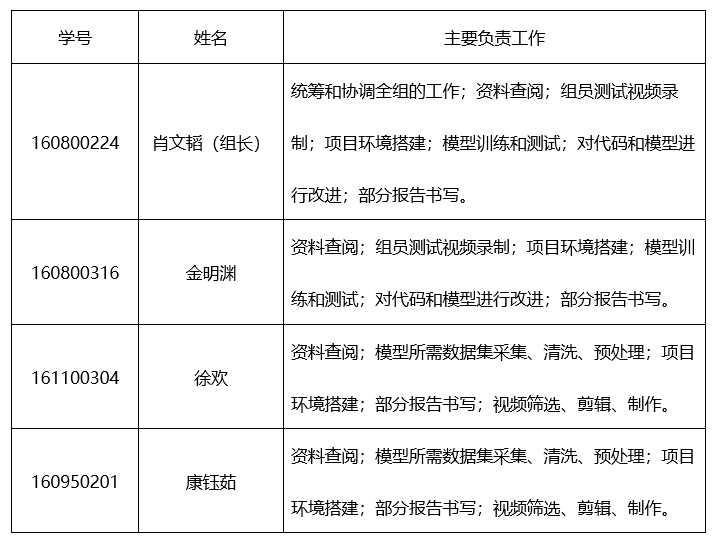
\includegraphics[width=\textwidth]{work_desc.png}
	\label{work_desc}
\end{figure}


我们组的工作总的来说是分为两部分的:第一部分是文献阅读和通用数据集测试,第二部分是提出改进思路以及在自制数据集上测试。

第一部分是在四月二十五号至五月十六号完成的,我们首先进行了大量及深刻的资料文件阅读和开源库的查找及使用。我们全体小组成员通过搜索引擎,Web Of Science 文献检索以及 Github,查阅和整理了所有有关人工智能换脸的论文和开源代码。在我们确定好主要参考的论文和开源代码之后,我们首先按照开源代码库中使用的通用数据集(特朗普和尼古拉斯凯奇数据集)进行了测试。为了测试上述数据集,我们首先需要做的就是搭建运行环境,我们先后在自己的电脑上面使用老师提供的外置显卡,以及在 Google 的免费科学计算平台 Colab 上面运行训练和测试。我们对测试结果和遇到的问题对代码和数据集进行了研究和修改。可以查看\textbf{表 \ref{work_1}}。


第一部分具体的工作时间线如下:

\begin{itemize}
	\item 4月25日。对象:全组。具体工作内容:确定项目;初步确定分工;查阅资料,寻找合适的代码库、数据集和有关论文。
	\item 4月26日-4月28日。全组。具体工作内容:明确分工细则;查阅资料,寻找合适的代码库、数据集和有关论文;初步确定项目所用算法(Faceswap),并对该算法进行学习和分析。
	\item 4月29日-5月2日。对象:全组。具体工作内容:深入分析和学习算法;寻找合适的服务器并初步测试核心代码;针对性修改代码中不适配的部分;寻找Faceswap的惯用数据集(Donald Trump和Nicolas Cage)并进行清洗和预处理。
	\item 5月3日-5月9日。对象:肖文韬,金明渊。具体工作内容:使用老师提供的GPU对Donald Trump和Nicolas Cage的数据集进行训练,得到模型后测试效果。对象:徐欢,康钰茹。具体工作内容:寻找合适的源视频,剪辑制作成测试视频,对训练所得模型进行测试。
	\item 5月10日-5月16日。对象:全组。具体工作内容:分析测试结果,将结果中效果不好的部分与代码进行对照,针对性修改代码和参数,制作更加适配的测试视频,得到较好结果;确定最终作品换脸对象(肖文韬和Emma Watson)。
\end{itemize}


第二部分是按照老师提出的建议。老师建议我们使用组员的视频素材作为测试数据,对通用数据集进行效果对比。具体的工作时间线如下:

\begin{itemize}
	\item 5月17日-5月23日。对象:肖文韬,金明渊。具体工作内容:分析当前所得模型的优点和缺点,通过查询资料和论文,寻找算法的改进方法,修改算法并进行初步测试;拍摄肖文韬同学的视频。对象:徐欢,康钰茹。具体工作内容:在网络上搜索下载Emma的照片,使用DeepFaceLab中的批处理文件,对换脸对象的视频进行固定帧数截屏,对以上所得图片进行人脸提取,进行数据清洗和预处理(筛选掉模糊/非人脸的照片素材, 得到合适大小的数据集)。
	\item 5月24日-5月30日。对象:肖文韬,金明渊。具体工作内容:使用老师提供的GPU,利用改进后算法对Emma和肖文韬的数据集进行训练,得到模型后测试训练效果;初步书写报告。对象:徐欢,康钰茹。具体工作内容:寻找合适的源视频,剪辑制作成测试视频,对训练所得模型进行测试;初步书写报告。
	\item 5月31日-6月5日。对象:全组。具体工作内容:分析测试结果,将结果中效果不好的部分与代码进行对照,针对性修改代码和参数,制作更加适配的测试视频,得到较好结果;完成报告的书写。
	\item 6月6日-6月13日。对象:全组。具体工作内容:制作PPT和视频。
\end{itemize}

\chapter{算法原理及流程}
\label{methodology}
在本章节中,我们首先介绍本实验的换脸框架的整体架构,然后对该架构中四个组成部分依次讲解。

\section{框架概览}
我们的 GAN 换脸框架的整体架构见 \textbf{图 \ref{fig:overall}}。

\begin{figure}[h!]
	\caption{框架概率}
	\centering
	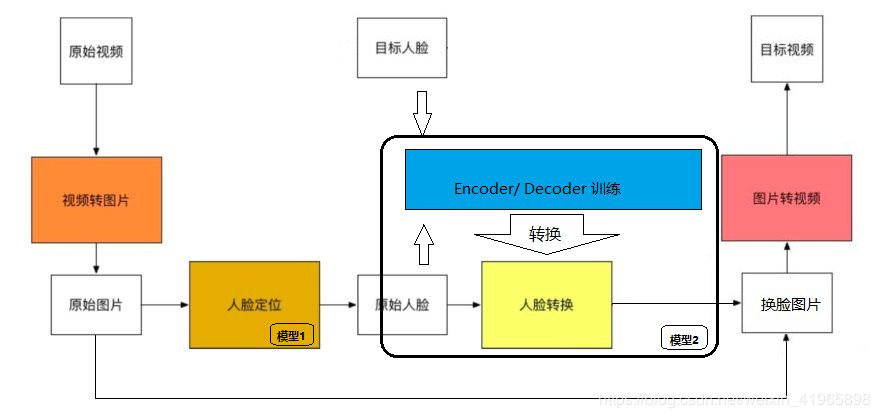
\includegraphics[width=\textwidth]{overall.jpg}
	\label{fig:overall}
\end{figure}

\section{人脸素材提取}
如果我们的原始数据是视频,我们首先将视频每间隔一定帧数(e.g.$6$ 帧)提取一帧得到一系列图片素材。
如果目标是公众人物我们也会使用搜索引擎搜集包含目标较为清晰的人脸的素材图片。
然后我们对这些素材图片使用 MTCNN 进行人脸识别提取出人脸部分的切图。
MTCNN 提取的是照片里面所有人脸的矩形坐标而这个矩形往往不是正方形因为我们的 GAN 模型输入输出都是正方形所以我们需要将这个矩形替换为相同面积相同位置的正方形区域。
此外因为人脸有多种角度所以我们需要首先将人脸规范化为标准正脸所以我们使用 MTCNN 输出的五个关键点(左右眼鼻子左右嘴角)的坐标信息使用 umeyama 函数将上述五个关键点坐标对应于标准正脸计算出来的关键点坐标生成一个在 2-D 欧式空间上的从原图关键点集到标准正脸关键点集的刚性对齐(rigid alignment)通俗的讲就是计算一个函数 $Tr(X)$ 能够通过缩放旋转变换操作使得 $\Vert Tr(X) - Y \Vert$ 尽可能小。
Umeyama是一种PCL算法,简单点来理解就是将源点云(source cloud)变换到目标点云(target cloud)相同的坐标系下,包含了常见的矩阵变换和SVD的分解过程。最终返回变换矩阵。计算过程与普氏分析极其相似。
提取出来的人脸实例及其对对齐之后的结果可以参考 \textbf{图 }。


因为 GAN 的训练需要两个目标 (A 和 B) 的人脸数据集所以人脸素材提取需要分别对两个目标进行提取。
提取素材需要注意:为了使模型的泛化能力更加好需要尽可能多地提取不同风格不同角度的照片作为素材并且有时候 MTCNN 提取出来的人脸切图是错误的压根就没有人脸。
并且对于区分度很低的相似照片也需要适当过滤掉。
这些都需要人工筛选。
数据集准则:


每个目标 $500$ 到 $5000$ 张人脸并且人脸需要是高质量含有各种角度,各种表情,各种关照条件的。


\section{眼部 Mask}
因为原来的 GAN 模型生成的视频眼部运动效果很不真实,所以在这个预处理环节,额外提取出眼部的 mask。
我们在这里使用 face alignment network 素材图片中提取眼部关键点(每个眼睛各有 $6$ 个关键点)。
对于每只眼睛,得到这几个关键点之后,我们从这几个关键点中生成闭包,然后再使用图形学膨胀使得这个闭合眼部 mask 过渡更加得自然,然后再使用高斯高通滤波进行除噪。
效果图可以参考 \textbf{图 \ref{fig:eyes_mask}},其中左边图片为一张人脸照片,右边的灰度图则为对应的眼部 mask 图片,白色表示眼部。

\begin{figure}[h!]
	\caption{眼部 mask 实例}
	\centering
	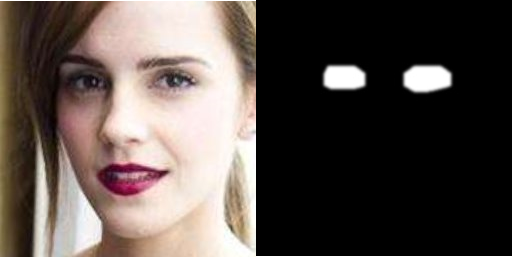
\includegraphics[width=\textwidth]{eyes_mask.png}
	\label{fig:eyes_mask}
\end{figure}

\section{生成式对抗网络}

\subsection{GAN 的组成}
GAN启发自博弈论中的二人零和博弈。在二人零和博弈中, 双方的利益之和为零或不变, 即一方有收益, 另一方必有损失。GAN模型中的两个参与者分别为生成模型G和判别模型D。
G捕捉样本的数据分布, D是一个二分类器, 估计样本训练数据的概率。G和D通常是非线性映射函数, 如卷积神经网络等,如 \textbf{图 \ref{fig:gan}} 所示。

\begin{figure}[h!]
	\caption{生成式对抗网络}
	\centering
	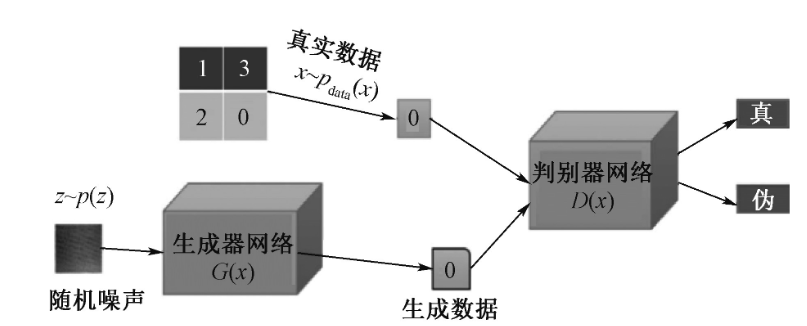
\includegraphics[width=\textwidth]{gan.png}
	\label{fig:gan}
\end{figure}


在GAN中, 第1个网络通常被称为生成器并且以G (z) 表示, 第2个网络通常被称为判别器并且以D (z) 表示。
判别器解决一个二分类问题并产生一个范围在0~1的直接标量。
在某种情况下, 这两个网络可以达到平衡点, 也就是极大极小博弈的最优点。第1个网络建模生成数据, 第2个网络认为第1个网络输出的结果是真实数据的概率为0.5, 但是在某种情况下却达不到, 两个网络会继续学习很长时间。


生成模型与对抗模型是完全独立的两个模型, 训练这两个模型的方法就是单独交替迭代优化训练, 优化过程是一个“二元极大极小博弈”问题。GAN最终需要优化的目标函数:

\begin{equation}
\min_G \max_D (E_{x \sim p_{data}(x)} [\log (D(x)) ] + E_{z \sim p_z(z)} [ \log (1 - D(G(z)))])
\end{equation}


这个目标函数既然是最大最小优化, 那就不是一步完成的, 先优化D, 然后优化G, 本质上是两个优化问题, 可拆解成式 (2) 和 (3) 再优化。


优化D:

\begin{equation}
\max_D (E_{x \sim p_{data}(x)} [ \log D(x) ] + E_{z \sim p_z(z)} [ log (1 - D(G(z)))])
\end{equation}


优化 G:

\begin{equation}
\min_G (E_{z \sim p_z(z)} [\log (1 - D(G(z)))])
\end{equation}


训练网络D使log D (x) 最大化, 以最大概率对其样本进行训练, 并使训练网络G最小化log (1-D (G (z) ) ) 。
在训练过程中固定一方, 更新另一方网络参数, 交替迭代, 使另一方的误差最大, 最后, G可以估计样本数据的分布。生成模型G隐式定义了概率分布Pg, 实际则希望Pg收敛到数据pdata的真实分布。GAN原始文献证明了这个极大极小博弈有一个最优解Pg=Pdata, 当其成立时即达到纳什均衡。

\subsection{数据增强}
在图像的深度学习中,为了丰富图像训练集,更好的提取图像特征,泛化模型(防止模型过拟合),一般都会对数据图像进行数据增强。数据增强,常用的方式,就是旋转图像,剪切图像,改变图像色差,扭曲图像特征,改变图像尺寸大小,增强图像噪音(一般使用高斯噪音,盐椒噪音)等。但是需要注意,不要加入其他图像轮廓的噪音。
如 \textbf{图 \ref{fig:data_aug}},对于人脸来说,使用扭曲的增强技术可以有效地降低训练过程中的损失值,当然增强也是有限度的,不要太过,物极必反。

\begin{figure}[h!]
	\caption{数据增强实例}
	\centering
	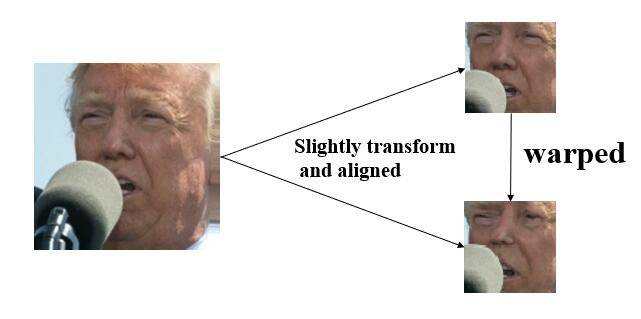
\includegraphics[width=\textwidth]{data_aug.jpg}
	\label{fig:data_aug}
\end{figure}

\subsection{自注意力机制}
因为传统 CNN 有感知域的问题,只擅长学习局部特征,如果要学习长距离依赖,必须堆叠很多层 CNN,这样的结果是模型庞大,收敛慢,容易出现梯度问题。
所以我们使用自注意力机制来学习长距离依赖。
我们使用 \citen{SAGAN}提出的自注意力机制对我们的模型进行改进。
\textbf{图 \ref{fig:sagan}} 展示了注意力机制用在卷积特征的过程。
传统的GAN模型都是在低分辨率特征图的空间局部点上来生成高分辨率的细节,而SAGAN是可以从所有的特征处生成细节,并且SAGAN的判别器可以判别两幅具有明显差异的图像是否具有一致的高度精细特征。SAGAN目前是取得了非常好的效果。
原因就在于这类模型依靠卷积来建立不同图像区域之间的依赖关系,而依赖关系的传递只能通过大范围的多个卷积层来实现。随着卷积大小的增加,网络的真实容量也在增加,但却损失了计算效率。而self-attentive,却能够做到依赖性和计算效率的平衡,因此文章引入self-attention机制

\begin{figure}[h!]
	\caption{自注意 GAN}
	\centering
	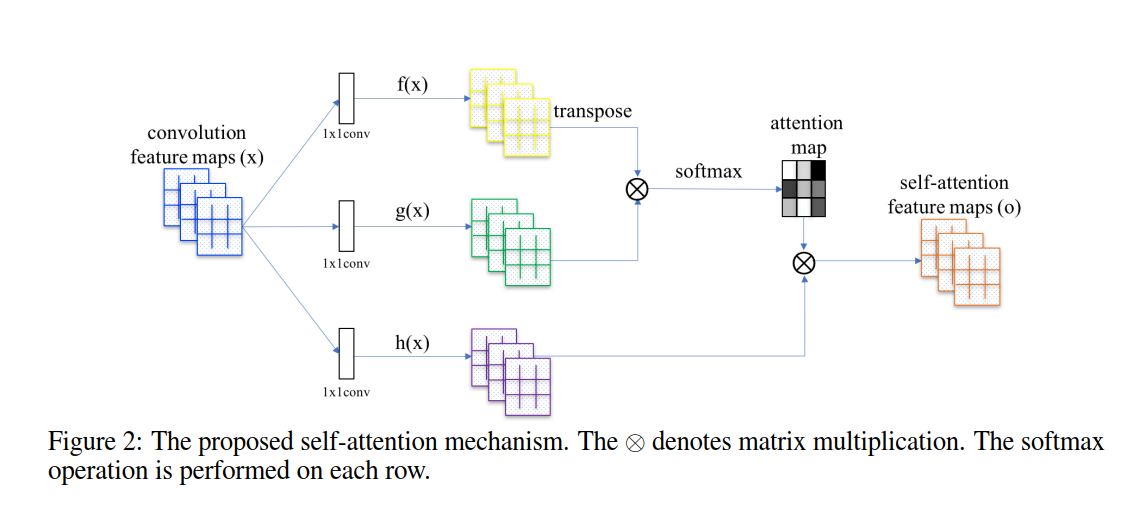
\includegraphics[width=\textwidth]{SAGAN.png}
	\label{fig:sagan}
\end{figure}


\subsection{CycleGAN}


\subsection{GAN}
该模型的生成器是一个编码解码器架构,其中编码器(\textbf{图 \ref{fig:encode}}) 学习一个人脸照片的中间表示,解码器 (\textbf{图 \ref{fig:decode}})将该中间表示解码为要生成的伪造人脸。

\begin{figure}[h!]
	\caption{编码器}
	\centering
	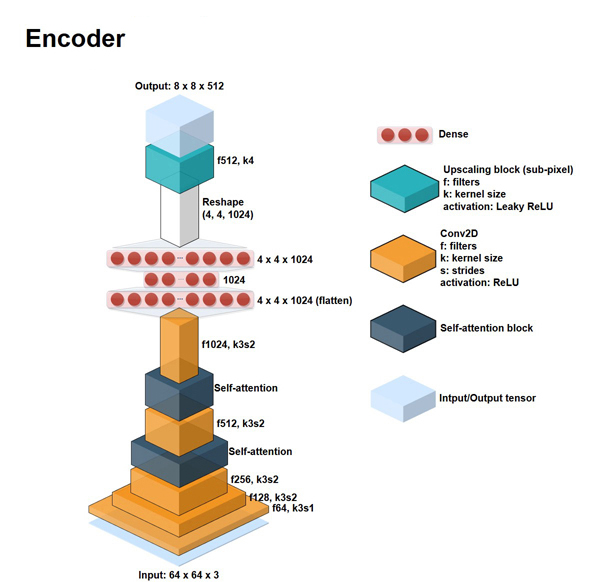
\includegraphics[width=\textwidth]{encode.jpg}
	\label{fig:encode}
\end{figure}

\begin{figure}[h!]
	\caption{解码器}
	\centering
	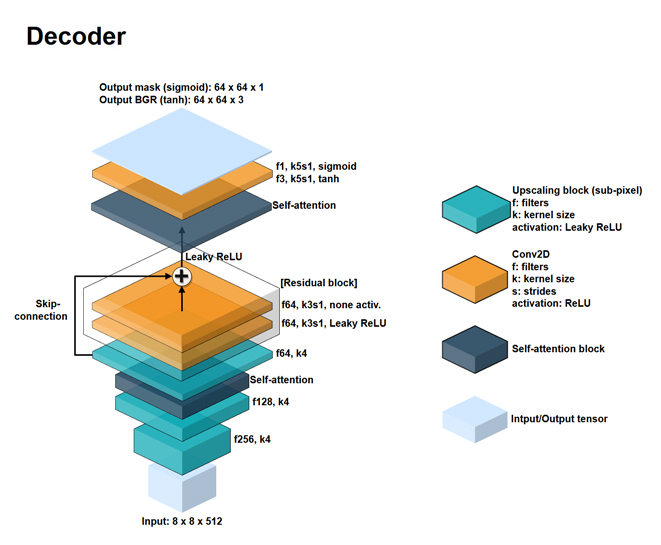
\includegraphics[width=\textwidth]{decode.jpg}
	\label{fig:decode}
\end{figure}

\begin{figure}[h!]
	\caption{判别器}
	\centering
	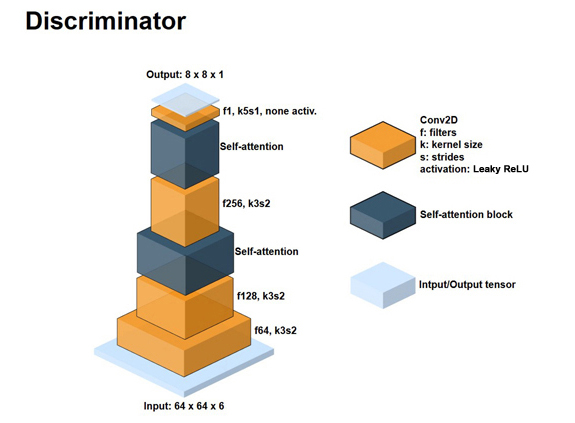
\includegraphics[width=\textwidth]{disc.jpg}
	\label{fig:disc}
\end{figure}

自编码器的简单例子可以看 \textbf{图 \ref{fig:encode_decode}}。

\begin{figure}[h!]
	\caption{自编码器的例子}
	\centering
	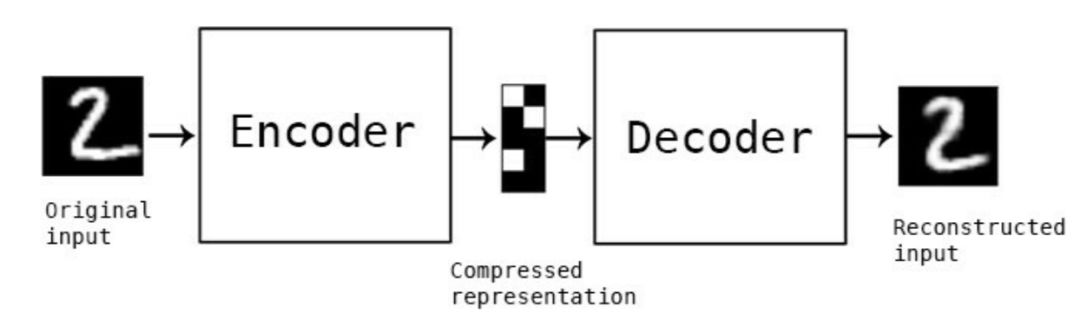
\includegraphics[width=\textwidth]{encode_decode.jpg}
	\label{fig:encode_decode}
\end{figure}

模型需要优化的损失函数在 \textbf{图 \ref{fig:loss}} 中展示。


\begin{figure}[h!]
	\caption{损失函数}
	\centering
	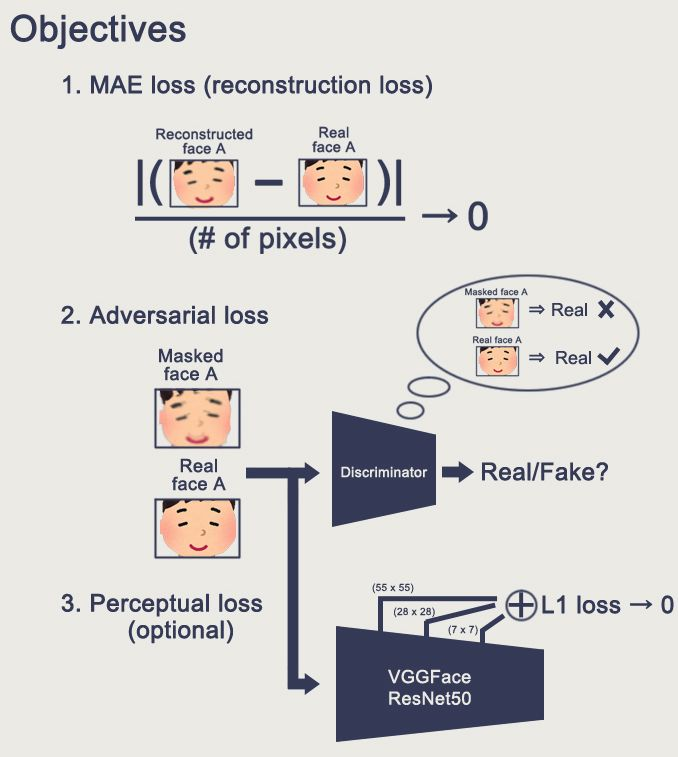
\includegraphics[width=\textwidth]{loss.jpg}
	\label{fig:loss}
\end{figure}


\section{视频换脸}
首先我们从视频中提取出所有的帧,对每一帧提取人脸图片然后喂给 GAN 生成针对另外一个目标的伪造图片。
由于生成出来的是一个正方形,如何与原图融合就是一个问题了,原始项目有很多种融合方法,包括直接覆盖,遮罩覆盖,还有就是泊松克隆「Seamless cloning」,从效果上而言,遮罩覆盖的效果与泊松克隆最好,二者各有千秋,遮罩覆盖边缘比较生硬,泊松克隆很柔和,其单图效果要优于遮罩覆盖,但是由于泊松克隆会使图片发生些许位移,因此在视频合成中会产生一定的抖动。

\chapter{改进方向:OctCNN}
卷积神经网络 (CNNs) 在许多计算机视觉任务中都取得了显著的成功,并且随着最近的研究在降低密集模型参数和特征图通道维数的固有冗余,它们的效率不断提高
然而,CNN 生成的特征图在空间维度上也存在大量冗余,其中每个位置独立存储自己的特征描述符,忽略了可以一起存储和处理的相邻位置之间的公共信息。
在自然的图像中,信息以不同的频率传递,其中较高的频率通常以精细的细节编码,较低的频率通常以全局结构编码。
类似地,卷积层的输出特征图也可以看做是不同频率的信息的混合。
\citen{OctCNN} 提出了一种新的多频特征表示方法,将高频和低频特征映射存储到不同的组中。
通过相邻位置间的信息共享,可以安全地降低低频组的空间分辨率,减少空间冗余。
作为传统卷积的替代,OctConv 消耗的内存和计算资源都大大减少。
此外,OctConv 利用相应的 (低频) 卷积处理低频信息,有效地扩大了原始像素空间的感受野,从而提高识别性能。
将卷积特征映射分解成不同空间频率的两个组,并分别以相应的频率处理不同的卷积,相隔一个八度 (octave)。由于可以降低低频图的分辨率,因此能够节省存储和计算。
这也有助于每一层获得更大的感受野,以捕获更多的上下文信息。
OctConv 直接对新的特征表示进行运算,减少了空间冗余。更重要的是,OctConv 在实践中速度很快,达到了接近理论极限的加速。
论文中广泛研究了所提出的 OctConv 在用于图像和视频任务的各种骨干 CNN 上的特性,并获得了显著的性能提高,甚至可以与最好的 AutoML 网络相媲美。


作为 CNN 的改进, OctCNN 即插即用无需调参,可以在实践中直接将 CNN 层替换为 OctCNN。
因此,我们将尝试用 OctCNN 替换掉 GAN 模型中的所有 CNN 层。
希望借此提高模型的训练速度和效果。

\chapter{实验结果及数据分析}
\label{experiments}

\section{实验过程}
针对这个模型,我们分别训练了两次,其中第一次是特朗普和尼古拉斯凯奇,第二次是肖文韬和emma。
在第一次模型训练之后,我们发现最终输出的视频结果还算客观,但是有以下问题:

\begin{enumerate}
	\item 最终视频换脸的素材不能与训练的样本差别太大,并且需要一定的分辨率(我们采用了720p的素材),不然换脸的结果会比较差。
	\item 最终结果可能呈现出不对称,即可能face A->face B效果较好,但face B->face A效果就不是很好。
	在第一次训练的背景下,我们重新采集了实验数据,确保了训练样本的多样化和高分辨率,然后进行了第二次训练。
	在第二次训练时,模型呈现了较高的收敛速度,经过40000代训练之后,双向的Adversarial loss已经分别达到了 0.15 和 0.14,而Reconstruction loss 均达到了0.20。
\end{enumerate}

\section{实验结果}
因为模型只能换面部特征,而没有考虑到头发,所以可能第一眼看上去换脸结果不太像,但是如果把头发遮掉的话就比较像。
第二次训练由于优化了训练集,所以最后的视频效果比第一次好。

最后的视频输出效果如下:


\chapter{总结与展望}
\label{conclusions}  
在本次工程实训的课程中,我们小组选择了GAN视频换脸这个项目,前期花了较多时间查阅各种资料和论文,对传统生成式对抗网络及之后相关技术的发展,如CGAN, pix2pix, CycleGAN等的创新和缺陷都有了初步的了解,对神经卷积网络也有了大概的认知。随后比对了网络上较为流行的视频换脸算法,对AI换脸的流程以及各个模型在其中的应用都有了更深层次的理解。

之前对于计算机行业的认知更多局限于软件开发相关,人工智能的概念虽然一直充斥于生活中,却没有真实接触过相关技术。因此此次实训是对我们知识储备的巨大提升,在惊叹于人工智能领域博大精深的同时,也激发了我们探索的兴趣。
此次实训是小组四人共同努力的结果,也走过选择了某个算法但发现效果一般于是重新筛选算法再进行训练的弯路。但最后的结果也还算令人满意,每个人都获得了成长,这次经历一定会成为宝贵的经验。

在实际进行模型测试的过程中,我们也发现了一些该算法的不足之处,并对它们进行了针对性的分析,尝试了对某些问题进行修改,如对在使用notebook进行训练的过程中,notebook假死的问题进行了debug,解决了这个问题。但由于每次训练模型的周期较长,约需要20小时左右,我们可以使用GPU的时间也较为有限,很多问题暂时还未得到解决,希望在今后能得到解决。当前算法训练模型过程中及训练出的模型还存在的未解决的问题主要有:
\begin{enumerate}
	\item 在训练过程中,每经过300iter,会输出当前训练的结果,以便对训练结果进行实时的监控,但代码中没有对此结果进行保存的部分,所以在训练结束后,若想对整个训练周期的各个阶段进行评估,并不是非常方便。日后希望能够在训练代码中加入将阶段性训练结果保存到指定文件夹的部分,以方便后期对照;
	\item 得到训练模型之后,输入视频进行换脸的测试,测试结果显示A->B和B->A的效果并不对称,如对Donald Trump和Nicolas Cage进行换脸,将Cage换成Trump的效果略好于将Trump换成Cage;对肖文韬同学和Emma Watson进行换脸,将Watson换成肖文韬的效果略好于将肖文韬换成Watson。这可能与训练模型过程中参数的调节有关,希望日后能通过不断的测试,加以改进;
	\item  得到成品视频之后,无法量化地评估换脸的效果,未来希望能够在输出测试结果之后,引入面部相似度的计算算法,量化地对换脸效果进行评估。如将视频中A的脸换成B,我们希望能够将换脸后的脸与B进行相似度对比;
\end{enumerate}

我们使用的算法,一个显著的优势是,在人脸检测和标定的步骤之后,使用了Face Alignment技术,在粗估计的形状的基础上,对眼部进行细化的特征点标记,在效果中的具体体现是,我们换脸后视频中,对眼部的置换格外精细,眼球转动置换的结果拟合度也非常高。未来如果能将Face Alignment的技术扩充到眼部以外的部分,如鼻子和嘴巴的部分,实现对全脸特征点的细化形状标定,得到的换脸效果必定更加稳定。

% \end{summary}

%% 附录
% \appendix
% %# -*- coding: utf-8-unix -*-
\chapter{搭建模板编译环境}

\section{安装TeX发行版}

\subsection{Mac OS X}

Mac用户可以从MacTeX主页\footnote{\url{https://tug.org/mactex/}}下载MacTeX 2015。
也可以通过brew包管理器\footnote{\url{http://caskroom.io}}安装MacTeX 2015。

\begin{lstlisting}[basicstyle=\small\ttfamily, numbers=none]
brew cask install mactex
\end{lstlisting}

\subsection{Linux}

建议Linux用户使用TeXLive主页\footnote{\url{https://www.tug.org/texlive/}}的脚本来安装TeXLive 2015。
以下命令将把TeXLive发行版安装到当前用户的家目录下。
若计划安装一个供系统上所有用户使用的TeXLive,请使用root账户操作。

\begin{lstlisting}[basicstyle=\small\ttfamily, numbers=none]
wget http://mirror.ctan.org/systems/texlive/tlnet/install-tl-unx.tar.gz
tar xzvpf install-tl-unx.tar.gz
cd install-tl-20150411/
./install-tl
\end{lstlisting}

\section{安装中文字体}

\subsection{Mac OS X、Deepin}

Mac和Deepin用户双击字体文件即可安装字体。

\subsection{RedHat/CentOS用户}

RedHat/CentOS用户请先将字体文件复制到字体目录下,调用fc-cache刷新缓存后即可在TeXLive中使用新字体。

\begin{lstlisting}[basicstyle=\small\ttfamily, numbers=none]
mkdir ~/.fonts
cp *.ttf ~/.fonts				# 当前用户可用新字体
cp *.ttf /usr/share/fonts/local/	# 所有用户可以使用新字体
fc-cache -f
\label{last}
\end{lstlisting}



\backmatter % 文后无编号部分
\printbibliography[heading=bibintoc]
\end{finish}

\end{document}
